\documentclass[12pt]{article}
\usepackage[serbian]{babel}


\usepackage{glossaries}
\usepackage{project}
\usepackage{glossary}
\usepackage{amsmath}
\usepackage{bytefield}
\usepackage{register}
\newcommand{\thesisName}{RaspberryPi generator funkcija sa AD9850 integrisanim kolom}
\newcommand{\subjectName}{Projekat iz predmeta Računarska Elektronika}

\author{Risto Pejašinović EE19/2015}
\newcommand{\mentor}{Prof.dr. Ivan Mezei}
\date{septembar 2019}


\begin{document}
\counterwithin{lstlisting}{section}
\counterwithin{figure}{section}
\counterwithin{equation}{section}
\counterwithin{table}{section}

\titlePageCmd

\noindent

\thispagestyle{empty}
\tableofcontents
\newpage
\newacronym{ui}{UI}{User Interface}
\newacronym{gui}{GUI}{Graphical User Interface}
\newacronym{cli}{CLI}{Command Line Interface}
\newacronym{sbc}{SBC}{Single Board Computer}
\newacronym{api}{API}{Application programming interface}
\newacronym{dds}{DDS}{Direct Digital Synthesis}
\newacronym{adc}{ADC}{Analog Digital Converter}
\newacronym{dac}{DAC}{Digital Analog Converter}
\newacronym{bash}{BASH}{Bourne Again SHell}
\newacronym{w_clk}{W\_CLK}{Data Write Clock}
\newacronym{fq_ud}{FQ\_UD}{Frequency Update}
\newacronym{rpi}{RPi}{RaspberryPi}

\printglossary[type=\acronymtype,style=mystyle]


\newpage


\section{Uvod}
Cilj ovog projekta je projektovanje preciznog i programabilnog generatora
sinusnog i pravougaonog signala sa jednostavnim \gls{ui}. \\
Potrebno je obezbediti jednostavan i intuitivan \gls{gui} i \gls{cli} korisnički interfejs.
\\

Za potrebne korisničkog interfejsa i zadavanja konfiguracije generatoru funkcija
odabran je \gls{sbc} \gls{rpi} pod GNU/Linux operativnim sistemom. \\
Za generisanje sinusnog i pravougaonog signala odabrano je AD9850 integrisano
kolo. \\

Cilj je obezbediti iste funkcionalnosti u \gls{gui} i \gls{cli} aplikaciji.
Ovo je postignuto korišćenjem jedinstvenog \gls{api} za AD9850 integrisao
kolo. Obe aplikacije trebaju implementirati pozive funkcija iz \gls{api}
.\\

\gls{cli} aplikacija omogućava podešavanje generatora funkcija pomoću skriptnih jezika
poput \gls{bash} i samim tim omogućava automatizaciju i proširenje
funkcionalnosti prema potrebi korisnika. Takođe korisnik može implementirati
dodatne funkcionalnosti u C++ jeziku korišćenjem AD9850 \gls{api}.

\subsection{AD9850}

AD9850 je integrisano kolo firme Analog Devices i koristi \gls{dds} tehnologiju
zajedno sa \gls{dac} i brzim komparatorom generiše precizan sinusni i
pravougaoni signal programabilne frekvencije visoke preciznosti. \\
Pravougaoni signal je generisan pomoću sinusne funkcije i komparatora.
Vreme ispune pravougaone funkcije se podešava analognim ulazom na komparatoru,
pa nije moguće digitalno podešavanje bez eksternih komponenti. \\

\begin{figure}[H]
  \centering{
    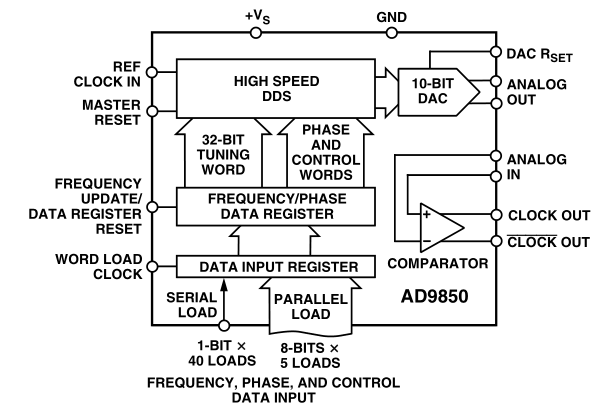
\includegraphics[width=10cm]{img/AD9850_bd.png}
  \caption{Funkcionalni dijagram AD9850\cite{AD9850_ds}}
  \label{func_bd_ad9850}
}
\end{figure}

Frekvencija se podešava postavljanjem 32-bitnog registra na željenu vrednost,
ovime je postignuta preciznost od 0.0291 Hz pri frekvenciji referentnog oscilatora od 125
MHz. \\
\gls{dds} omogućava frekvenciju to polovine referentnog takta, ali je \gls{dac}
ograničava na 40 MHz.
Pored podešavanje frekvencije moguće je i podešavanje faze između dva analogna
izlaza. \\

Moguća je promena izlazne frekvencije brzinom do 23 miliona
novih frekvencija u sekundi.
Ova brzina će zavisiti od načina upisivanja u konfiguracioni registar.
Moguće je upisivati konfiguraciju serijski ili 8-bita paralelno.
U slučaju serijskog upisa potrebno je upisati 40-bita što će oduzeti 40 upisnih
taktova, prilikom paralelnog upisa potrebno je 5 upisnih taktova. \\

\subsubsection{Reset sekvenca}
Pre učitavanja konfiguracionog registra potrebno je resetovati AD9850.
Kako bi se AD9850 resetovao potrebno je generisati sekvencu kao na slici(\ref{ad9850_rst_seq}). \\

\begin{figure}[H]
  \centering{
    \scalebox{1.2}{
      \\
\begin{tikztimingtable}[%
  timing/dslope=0.1,
  timing/.style={x=5ex,y=2ex},
  x=5ex,
  timing/rowdist=4ex,
  timing/name/.style={font=\sffamily\scriptsize}
  ]
  \busref{RST}      & 1u 1L 1H 4L U \\
  \busref{W\_CLK}   & 1u 2.5L 1H 2.5L U \\
  \busref{FQ\_UD}   & 1u 4.0L 1H 1.0L U \\
  \busref{DATA}     & 4U 1L 2.5L  \\
  \extracode
  \begin{pgfonlayer}{background}
  \end{pgfonlayer}
\end{tikztimingtable}
    }}
  \caption{Reset sekvenca}
  \label{ad9850_rst_seq}
\end{figure}

Nakon resetovanja AD9850 je spreman za prihvatanje konfiguracije i generisanje signala.
Sekvencu za neophodno generisati prilikom uspostavljanja napajanja, dok prilikom promene
konfiguracije reset nije neophodno odraditi.

\subsubsection{Konfiguracioni registar}

AD9850 se u potpunosti upravlja preko jedno 40-bitnog registra u kojem su
sadržana frekvencija signala, faza i kontrolni bitovi.

\begin{register}{H}{Konfiguracioni registar}{}% name=example
  \label{example}%
  \regfield{Freq B4}{8}{32}{{Freq b31-b24}}%
  \regfield{Freq B3}{8}{24}{{Freq b23-b16}}%
  \regfield{Freq B2}{8}{16}{{Freq b15-b8}}%
  \regfield{Freq B1}{8}{8}{{Freq b7-b0}}%
  \regfield{Phase}{5}{3}{{Phase b4-b0}}%
  \regfield{Power}{1}{2}{{PD}}%
  \regfield{Control}{2}{0}{{Control}} \\
  \begin{regdesc}\begin{reglist}[Request~Depth]
    \item [Freq B4-B1] Podešava izlaznu frekvenciju generatora.\\
      Vrednost ovog registra može se dobiti sledećom formulom:
      \[
      Freq [31:0] = \frac{freq*2^3^2}{DDS\_CLK}
      \] \\
      freq je željena frekvencija, DDS\_CLK je referentni takt.
    \item [Phase] Podešava fazu.
    \item [Power] Kada je ovaj bit setovan na jedinicu AD9850 je u Power-Down modu.
    \item [Control] Treba biti 0 kako bi oba \gls{dac} izlaza bila aktivna.
    \end{reglist}\end{regdesc}
\end{register}

\subsubsection{Sekvenca za učitavanje konfiguracije}

Nakon uspešnog resetovanja potrebno je upisati željenu konfiguraciju.
Upisivanje u serijskom modu je prikazano na slici (\ref{ad9850_load_seq}).

\begin{figure}[H]
  \centering{
    \scalebox{1.1}{
      \\
\newcommand{\strobeSig}{0.25L 0.5H 0.25L}
\begin{tikztimingtable}[%
  timing/dslope=0.1,
  timing/.style={x=5ex,y=2ex},
  x=5ex,
  timing/rowdist=4ex,
  timing/name/.style={font=\sffamily\scriptsize}
  ]
  \busref{RST}      & 1u 12L \\
  \busref{DATA}     & 1u 1L 1D{Freq b0} 1D{Freq b1} ;[dotted]1D{b2-30}; 1D{Freq b31} 1D{Ctrl b0}
  1D{Ctrl b1} 1D{Power} 1D{Ph b0} ;[dotted]1D{b1-3}; 1D{Ph b4} 1L \\
  \busref{W\_CLK}   & 1u 1L \strobeSig \strobeSig ;[dotted]1L; \strobeSig
  \strobeSig \strobeSig \strobeSig \strobeSig ;[dotted]1L; \strobeSig L \\
  \busref{FQ\_UD}   & 1u 11L \strobeSig \\
  \extracode
  \begin{pgfonlayer}{background}
  \end{pgfonlayer}
\end{tikztimingtable}
    }}
  \caption{Sekvenca serijskog učitavanja}
  \label{ad9850_load_seq}
\end{figure}

Za detaljne informacije o tajminzima pogledati datasheet \cite{AD9850_ds}.

\newpage

\subsubsection{AD9850 modul}

Na slici \ref{ad9850_mod_pinout} prikazan je raspored pinova AD9850 modula
korišćenog u ovom projektu. \\

\begin{figure}[H]
  \centering{
    \includegraphics[width=10cm]{img/AD9850_module.jpg}
    \caption{Raspored pinova AD9850 modula\cite{AD9850_module_pinout}}
    \label{ad9850_mod_pinout}
  }
\end{figure}


Pinove označene sa prefiksom Serial je potrebno koristiti u slučaju serijske
komunikacije. \\
Pinovi obeleženi sa DX se koriste za paralelno upisivanje i u ovom slučaju mogu
se ostaviti nepovezani. \\
Plavom strelicom su označeni izlazni pinovi, od kojih su dva za pravougani
signal dva za sinusni. \\

Na ploči se nalazi referentni oscilator od 125 MHz. \\

Na ulaz internog komparatora za generisanje pravougaonog signala je doveden
napon sa potenciometra na slici, ovo omogućava ručno podešavanje vremena ispune
pravougaonog signala.
Na žalost ovaj modul ne dozvoljava programabilno podešavanje vremena ispune
pravougaonog signala. \\

\newpage

\section{Aplikacija}

\subsection{Režimi rada}\label{working_modes}
Kao što je već rečeno \gls{cli} i \gls{gui} aplikacija trebaju da obezbede iste
funkcionalnosti.\\
Režimi rada koji su implementirani u ovom projektu su opisani u nastavku.
\begin{itemize}
\item \label{run_mode} \textbf{Run} pokretanje generatora sa fiksnom frekvencijom bez vremenskog
  ograničenja rada, potreban argument:
  \begin{itemize}
    \item \textbf{freq} zadata frekvencija generisanog signala u Hz.
  \end{itemize}
\item \label{run_for_mode} \textbf{Run for} pokretanje generatora sa fiksnom frekvencijom sa
  određenim vremenom trajanja.
  \begin{itemize}
  \item \textbf{freq} zadata frekvencija generisanog signala u Hz.
  \item \textbf{time\_ms} trajanje generisanja signala u ms.
  \end{itemize}

\item \label{sweep_mode} \textbf{Sweep} linearna promena frekvencije između dve definisane
  vrednosti.
  \begin{itemize}
  \item \textbf{start\_freq} početna frekvencija u Hz.
  \item \textbf{stop\_freq}  krajnja frekvencija u Hz.
  \item \textbf{step\_freq}  vrednost koraka frekvencije u Hz.
  \item \textbf{step\_time}  vreme zadržavanja na svakom koraku u ms.
  \end{itemize}
  Ovaj režim rada generatora se često koristi u ispitivanju frekvencijskih karakteristika
  elektronskih kola ili komponenti.
  Za prikazivanje frekvencijske karakteristike na osciloskopu, pored signala promenljive
  frekvencije potrebno je obezbediti i trougaoni signal kao izvor vremenske baze
  osciloskopa. \\
  Ovakav uređaj se naziva Sweep Generator ili Wobbler.
  Često se jedan kanal osciloskopa može koristiti kao izvor vremenske baze dok
  drugi služi kao ulaz za Y-osu.

\end{itemize}

\subsubsection{Konfiguracija aplikacije} \label{config_file}
Potrebno je obezbediti mogućnost promene pinova preko kojih je \gls{rpi} povezan
sa AD9850 modulom bez ponovnog kompajliranja aplikacije.
Takođe ovo podešavanje treba da bude zajedničko za CLI i GUI aplikaciju.\\
Ovo je rešeno korišćenjem deljenog konfiguracionog fajla. \\

\noindent
Konfiguracioni fajl treba da sadrži sledeće parametre.
\begin{itemize}
\item \textbf{w\_clk} broj WiringPi pina povezanim sa \textbf{W\_CLK} pinom na AD9850 modulu.
\item \textbf{fq\_ud} broj WiringPi pina povezanim sa \textbf{FQ\_UD} pinom na AD9850 modulu.
\item \textbf{data} broj WiringPi pina povezanim sa \textbf{D7} pinom na AD9850 modulu.
\item \textbf{rst} broj WiringPi pina povezanim sa \textbf{RST} pinom na AD9850 modulu.
\item \textbf{dds\_clk} frekvencija referentnog oscilatora u Hz na AD9850 modulu.
\end{itemize}

Na \textbf{GNU/Linux} operativnim sistemima konfiguracioni fajlovi se trebaju
nalaziti u definisanom deljenom direktorijumu. \\
Prema \textbf{XDG Base Directory Specification}\cite{xdg_spec} od freedesktop projekta
treba se poštovati sledeće pravilo za skladištenje konfiguracionih fajlova.

\begin{itemize}
  \item Ukoliko je promenljiva okruženja \textbf{XDG\_CONFIG\_HOME} postavljena,
    tada ona sadrži putanju direktrijuma gde se smeštaju korsnički
    konfiguracioni fajlovi za aplikacije.
  \item Ukoliko promenljiva okruženja \textbf{XDG\_CONFIG\_HOME} nije postavljena, kao
    direktorijum za smeštanje korisničkih konfiguracionih fajlova treba
    koristiti \textbf{\$HOME/.config}.
  \item Svaka aplikacija koja ima potrebe za konfiguracionim fajlom treba imati
    svoj direktorijum unutar \textbf{XDG\_CONFIG\_HOME} direktorijuma gde će se
    nalaziti konfiguracioni fajlovi.
\end{itemize}

Ovo ne deluje kao previše bitna stavka, ali bi poštovanje ovih pravila trebalo
biti obavezno.
Zbog nepoznavanje ove specifikacije od strane programera nastali su programi
koji nemaju zajednički direktorijum za konfiguracione fajlove, već se oni mogu naći
svuda po sistemu.
Ovo stvara problem prilikom backup-ovanja sistema, ukoliko su svi konfiguracioni
i korisnički fajlovi na definisanom mestu backup sistema može biti automatizovan i siguran. \\
Ova specifikacija definiše direktorijume i za ostale korisničke fajlove. \\

Potrebno je na siguran način parsirati i upisivati ove konfiguracione fajlove.
Kako bi se izbeglo ponovno pisanje ovakve biblioteke i izbegli rizici za ovaj projekat izabrana je \textbf{libconfig}\cite{libconfig} biblioteka.\\

Za pristup GPIO pinova RPi korišćena je WiringPi\cite{WiringPi} biblioteka

\subsection{Uputstvo za instalaciju}

Kako bi se aplikacija uspešno kompajlirala potrebno je prvo instalirati potrebne
pakete i biblioteke koje se koriste u ovom projektu. \\
Korišćeni paketi bi trebali biti dostupne na repozitorijumu svake poznatije Linux
distribucije. \\
U ovom slučaju je korišćena Arch Linux ARM distribucija pa će za nju biti
opisana instalacija paketa.

\begin{lstlisting}[language=bash, basicstyle=\normalsize]
  $ pacman -S qt5-base libconfig
  $ yay -S wiringpi-git
\end{lstlisting}

U ovom slučaju koristi se \textbf{yay AUR helper} za pristup AUR repozitorijumu.
Ukoliko je potrebna samo CLI aplikacija \textbf{qt5-base} paket nije potreban.\\
\newpage

Nakon ovoga potrebno je klonirati git repozitorijum ovog projekta

\begin{lstlisting}[language=bash, basicstyle=\normalsize]
  $ git clone https://github.com/Risto97/ad9850_rpi
  $ cd ad9850_rpi
  $ make
\end{lstlisting} %$

Opciono može se pokrenuti \textbf{sudo make install} kako bi se aplikacija instalirala u \textbf{/usr/bin}
direktorijumu. U suprotnom izvšni fajl će se nalaziti u \textbf{bin} direktorijumu
kloniranog git repozitorijuma. \\

Ukoliko je potrebna samo CLI ili GUI aplikacija može se uraditi \textbf{make cli\_app}
ili \textbf{make gui\_app}. Za dokumentaciju potrebno je izvršiti \textbf{make docs}.

\subsection{CLI aplikacija}

\gls{cli} je aplikacija koja se izvršava bez grafičkog okruženja preko komandne linije.
Ovo je često bolji pristup za određene aplikacije.
Kod nekih aplikacija grafičko okruženje nije neophodno i često ih je
lakše i pouzdanije upravljati preko komandne linije. \\

\subsubsection{Prednosti CLI aplikacije}
CLI aplikacije su manje kompleksne od GUI aplikacija i
samim tim postoji manje mogućnosti za postojanje bug-ova.
Funkcionalnost programa je najčešće bitnija od grafičkog interfejsa,
jednostavnost CLI aplikacije omogućava programeru da se fokusira više na samu
funkcionalnost. \\

Dodatna prednost CLI aplikacije je lakše pokretanje i podešavanje iz
skriptnih jezika (BASH, Python) ovo često kod GUI aplikacija nije moguće.
Skriptovanje omogućava automatizaciju poslova i uklanja potrebu za ljudskim faktorom.\\

\subsubsection{Parsiranje argumenata komandne linije}

Jedan od zadataka CLI aplikacije je parsiranje argumenata komandne linije.
Kako bi se skratilo vreme razvoja i izbegla mogućnost grešaka može se koristiti
neka od biblioteka za parsiranje argumenata, u ovom projektu je korišćena
\textbf{cxxxopts}\cite{cxxopts} biblioteka.

Ova biblioteka se sastoji samo od jednog Header fajla, time uklanja potrebu za
kompajliranjem dodatne biblioteke.
\newpage

\subsubsection{Uputstvo za upotrebu}

Pokretanjem \textbf{ad9850\_cli} izvršnog fajla sa argumentom \emph{---help} na
\textbf{stdout} će se ispisati uputstvo za upotrebu. \\

\begin{lstlisting}[language=bash, caption=ad9850\_cli help opcija]
   $ ad9850 --help
   AD9850 cli application.
   Usage:
     AD9850 [OPTION...]

         --run arg        Run with frequency arg
         --run-for arg    Run with frequency arg[0] for time arg[1] in ms
         --sweep arg      Sweep from freq arg[0] to freq arg[1] with step freq
                          arg[2] and step time arg[3] in Hz and ms
         --stop           Stop ad9850
         --read-cfg       Prints tuple of configuration parameters to stdout
         --write-cfg arg  Write cfg, arg is tuple = w_clk,fq_ud,data,rst,dds_clk
         --help           Show help

\end{lstlisting} %$

Na osnovu uputstva možemo pokrenuti generator u Sweep režimu na sledeći način.

\begin{lstlisting}[language=bash, caption=ad9850\_cli sweep opcija]
  $ ad9850 --sweep 1000,10000,100,10
  Sweeping from 1000 Hz to 10000 Hz, with step 100 Hz and step time 10 ms
\end{lstlisting} %$
\subsection{GUI aplikacija}

Napisana je pomoću Qt Framework-a \cite{qt}. \\
Za GUI aplikaciju potrebno je obezbediti intuitivan i jednostavan interfejs.
Potrebno je obezbediti pristup svim režimima rada navedenim u sekciji
\ref{working_modes}. \\
Pored toga treba implementirati ispisivanje i promenu konfiguracionog fajla odnosno
promenu pinova preko kojih RPi pristupa AD9850 modulu i frekvenciju referentnog takta.

\subsubsection{Opis dizajna}
Za potrebe ovog projekta osmišljen je sledeći dizajn. \\
Glavni prozor aplikacije je podeljen na dva \textbf{Widget}-a \cite{QWidget}.
Levi Widget je klase \textbf{QTabWidget} koji podržava kartice. \\
Desni widget je fiksan i prikazuje statusne informacije, na njemu se još nalazi
i taster za zaustavljanje generatora. \\
Na glavnom prozoru se nalazi još i \textbf{QMenu}\cite{QMenu}, preko kojeg se
može pokrenuti dijalog za pristup konfiguracionom fajlu koji je prikazan na
slici(\ref{config_dialog}). \\

Widget sa karticama trenutno sadrži Basic i Sweep karticu. Basic kartica
prikazana na slici(\ref{basic_tab}) pokriva
\textbf{Run} i \textbf{Run for} režime rada. \\
Sweep kartica prikazana na slici(\ref{sweep_tab}) pokriva \textbf{Sweep}
režim rada. \\

Organizacijom ovog widget-a pomoću kartica ostavlja se mogućnost proširenja programa
sa novim režimima rada, a da se pritom ne narušava dizajn interfejsa i izbegne
prenatrpanost. \\


\subsubsection{Basic kartica}

Kao što se vidi na slikama(\ref{basic_tab}, \ref{basic_tab2}), ova kartica se
sastoji iz dva polja za unos, realizovani pomoću QSpinBox\cite{QSpinBox} klase i
dva tastera QPushButton\cite{QPushButton} klase. \\

Tasteri \textbf{Start} i \textbf{Run For} pokreću generator u režimima \textbf{Run} odnosno \textbf{Run For}. \\
U slučaju režima \textbf{Run} razmatra se samo polje za unos sa opisom
\textbf{Frequency}. \\
U slučaju režima \textbf{Run For} potrebno je uneti vremensko trajanje rada generatora u
polje za unos sa opisom \textbf{Run Time}. \\
\begin{figure}[H]
  \centering{
    \includegraphics[width=10cm]{img/AD9850_gui_run.png}
    \caption{AD9850 GUI Basic Tab}
    \label{basic_tab}
  }
\end{figure}

\begin{figure}[H]
  \centering{
    \includegraphics[width=10cm]{img/AD9850_gui_run_for.png}
    \caption{AD9850 GUI run for}
    \label{basic_tab2}
  }
\end{figure}

\subsubsection{Sweep kartica}

Na slici(\ref{sweep_tab}) prikazana je Sweep kartica, ona se sastoji iz četiri
polja za upis i tastera Sweep. \\
Opisi parametara u ovom režimu se nalaze u sekciji(\ref{working_modes})

\begin{figure}[H]
  \centering{
    \includegraphics[width=10cm]{img/AD9850_gui_sweep.png}
    \caption{AD9850 GUI Sweep Tab}
    \label{sweep_tab}
  }
\end{figure}

\subsubsection{Status widget}

Potrebno je da korisnik ima uvid u trenutno stanje generatora, u tu svrhu je
napravljen Status widget koji se nalazi sa desne strane interfejsa.
Može se videti na slikama(\ref{basic_tab}, \ref{basic_tab2}, \ref{sweep_tab}).
\\
Na njemu se nalazi QLabel\cite{QLabel} koji prikazuje trenutni režim u kojem
generator radi i njegove parametre, QLedIndicator\cite{QLedIndicator}
predstavlja indikator da li je generator aktivan ili nije i taster za stopiranje generatora.


\subsubsection{Dijalog za konfiguraciju}

Dijalogu za konfiguraciju može se pristupiti preko config menija na glavnom
prozoru, prikazan je na slici(\ref{config_dialog}). \\
Sastoji se od četiri \textbf{QComboBox}\cite{QComboBox} padajućih prozora u
kojima se nalaze brojevi dostupnih pinova prema \textbf{WiringPi} biblioteci, jednog
\textbf{QSpinBox} polja za unos frekvencije referentnog oscilatora i dva tastera. \\

Prilikom pokretanja ovog dijaloga čita se konfiguracioni fajl opisan u
sekciji(\ref{config_file}), zatim prikazuje pročitane parametre u odgovarajućim
poljima. \\

Nakon promene vrednosti padajućih prozora ili polja za unos moguće je sačuvati
promene u konfiguracioni fajl pritiskom na taster \textbf{Save config}. \\
Pritiskom na taster \textbf{Ok} aplikacija učitava novo podešene parametre. \\

\begin{figure}[H]
  \centering{
    \includegraphics[width=6cm]{img/AD9850_gui_cfg.png}
    \caption{AD9850 konfiguracioni dijalog}
    \label{config_dialog}
  }
\end{figure}


\section{Zaključak}

Razvijena aplikacija omogućava jednostavno upravljanje osnovnim režimima rada
AD9850 integrisanog kola. \\
RPi se pokazao kao dobra platforma za razvoj korisničkog interfejsa generatora
funkcija i ostavlja mogućnost za lako proširenje funkcionalnosti. \\

\subsubsection{Predlozi proširenja}
U nastavku biće predloženi načini na za proširenje ovog projekta.
Implementacijom ovih predloga može se dobiti uređaj u oblasti audio elektronike
i drugih oblasti na višim frekvencijama. \\
Većina ovih predloga zahteva projektovanje dodatnih analognih
elektronskih kola pa zbog toga njihova implementacija nije razmatrana u ovom projektu. \\

\begin{itemize}
\item \textbf{Dodavanje izlaznog pojačavača} signala sa mogućnosti dodavanja napona
  offset-a kako bi se obezbedili standardni naponski nivoi prisutni kod
  komercijalnih generatora funkcija (+,- 15V). \\
  Zbog relativno širokog opsega frekvencija generisanog signala (0-40MHz) ovo
  nije trivijalan zadatak i potrebno je korišćenje odgovarajućeg operacionog
  pojačavača sa dovoljno širokim frekventnim opsegom, alternativno ograničiti
  izlaznu frekvenciju na uži opseg.

\item \textbf{Softversko podešavanje ispune pravougaonog signala}. \\
  Modul korišćen u ovom projektu nema spoljni pristup ulazu internog komparatora i
  potrebno je izvršiti modifikaciju na ploči ili projektovati novu ploču.
  Potrebno je obezbediti analogni napon sa mogućnosti podešavanja softverskim
  putem, najverovatnije korišćenjem integrisanog \textbf{AD} konvertora.

\item \textbf{Proširenje projekta na Wobbler generator}. \\
  Realizovan sweep režim rada predstavlja osnovu Wobbler generatora. \\
  AD9850 je pogodan za realizaciju ovog uređaja zbog širokog opsega izlazne
  frekvencije i mogućnost brze promene frekvencije. \\
  Pored Sweep signala potrebno je obezbediti i trouglasti signal za vremensku
  bazu osciloskopa kao i potrebne pojačavače za oba signala.

\end{itemize}

\subsubsection{Slike rada}

U nastavku su okačene slike sa logičkog analizatora koje prikazuju rad uređaja.

\newpage

\bibliography{bibliography}
\bibliographystyle{IEEEtran}

\end{document}